\documentclass{article}
\usepackage[utf8]{inputenc}
\usepackage[a4paper, portrait, margin=0.75in]{geometry}

\usepackage{amsmath}
\usepackage{amsthm}
\usepackage{amssymb}

\usepackage{tikz}
\usetikzlibrary{arrows.meta}
\usetikzlibrary{decorations.markings}

\newcommand{\diff}{\mathop{}\!\mathrm{d}}
\newcommand{\R}{\mathbb{R}}
\newcommand{\C}{\mathbb{C}}
\newcommand{\principalvalue}{\text{p.v.}}

\theoremstyle{definition}
\newtheorem{defn}{Defn}[section]
\newtheorem{thm}{Theorem}[section]
\newtheorem{corl}{Corollary}[section]

\begin{document}

\tableofcontents

\pagebreak

\tikzset{
	arrow along/.style={
		thick,
		decoration={
			markings,
			mark=at position 0.5 with{
				\arrow{latex};
			}
		},
		postaction={decorate}
	}
}

% -------------------- Notation

\section{Notation}
\begin{itemize}
	\item $I = [0,1]$ the unit interval.
	\item $C^\infty(M)$ the set of smooth functions $f : M \to \R$ on a manifold $M$.
	\item $\mathfrak{X}(M)$ the set of smooth vector fields on $M$.
\end{itemize}

% -------------------- Vector Calculus

\section{Vector Calculus}
\subsection{Divergence and Stokes Theorem for Scalar Functions}
Let $f \in C^\infty(\R)$. We wish to integrate $f$ over some volume $V \subset \R^3$. 
Introduce constant vector field $\vec{c} \in \mathfrak{X}(\R^3)$, and consider
the new vector field $\vec{F} = f \vec{c}$. Applying the divergence theorem:
\begin{equation*}
\begin{split}
	\int_V \nabla \cdot \vec{F} \diff^3 r &= \int_{\partial V} \vec{F} \cdot \diff\vec{S} \\
	\vec{c} \cdot \int_V \nabla f \diff^3 r &= \vec{c} \cdot \int_{\partial V} f \diff\vec{S} \\
	\int_V \nabla f \diff^3 r &= \int_{\partial V} f \diff\vec{S} \\
\end{split}
\end{equation*}

For a vector field $\vec{A} \in \mathfrak{X}(\R^3)$, we may repeat the process to
derive a corresponding Stokes' theorem:
\begin{equation*}
	\int_V \nabla \times \vec{A} \diff^3 r = \int_{\partial V} \diff\vec{S} \times \vec{A}
\end{equation*}

% -------------------- Integration Techniques

\section{Integration Techniques}

\subsection{Contour Integration}
Let $z : I \to \C$ be a curve defining the contour $C \subset \C$ in the complex plane.
Consider the integral of a complex function $w(z) = u(x,y) + iv(x,y)$ where
$z(t) = x(t) + iy(t)$. We may write it as a linear combination of real integrals:
\begin{equation*}
\begin{split}
	\int_C w(z) \diff z
		&= \int_C (u \diff x - v \diff y) + i \int_C (v \diff x + u \diff y) \\
		&= \int_0^1 \left(u \frac{dx}{dt} - v \frac{dy}{dt}\right) \diff t + i \int_0^1 \left(v \frac{dx}{dt} + u \frac{dy}{dt}\right) \diff t \\
\end{split}
\end{equation*}

\begin{thm}[Cauchy-Goursat]
	If $f(z)$ is analytic wihtin and on a contour $C$, then
	\begin{equation*}
		\oint_C f(z) \diff z = 0
	\end{equation*}
\end{thm}
\begin{corl}[Path Independence]
	If $f(z)$ is analytic within a region $R$, and $C_1,C_2$ lie within $R$ with the same
	endpoints, then
	\begin{equation*}
		\int_{C_1} f \diff z = \int_{C_2} f \diff z
	\end{equation*}
	(c.f. path independence of conservative vector fields) 
\end{corl}

\textbf{Example}: Integral of $1/z$ along the unit circle. \\
Let $f(z) = 1/z$, and $C$ be the unit circle in the complex plane. Rewriting
$z = e^{i\theta}$ along the unit circle:
\begin{equation*}
	\int_C \frac{\diff z}{z} = \int_0^{2\pi} \frac{\diff \left(e^{i\theta}\right)}{e^{i\theta}} \diff \theta = i \int_0^{2\pi} \diff \theta = 2\pi i
\end{equation*}

\begin{thm}[Cauchy Integral Formula]
	If $f(z)$ is analytic within and on a closed contour $C$, then for any $z_0$ interior
	to $C$,
	\begin{equation*}
		f(z_0) = \frac{1}{2\pi i} \oint_C \frac{f(z)}{z - z_0} \diff z
	\end{equation*}
	Proof outline: deform $C$ to an arbitrarily small circle about $z_0$. Then $f(z)
	= f(z_0) + (f(z) - f(z_0))$ with a factor of $2\pi i$ coming from integrating
	$1/z$. The error term $f(z) - f(z_0)$ vanishes along an arbitrarily small circle. 
\end{thm}
This may be used to calculate the $n$th derivative of an analytic function:
\begin{equation*}
	f^{(n)}(z_0) = \frac{n!}{2\pi i} \oint_C \frac{f(z)}{(z-z_0)^{n+1}} \diff z
\end{equation*}

\subsection{Principal Value}
Consider a function $f(z)$, analytic in the upper half of the complex plane, which
satisfies $|f(z)| \to 0$ as $|z| \to \infty$. Consider the contour integral
\begin{equation*}
	\oint_C \frac{f(z)}{z - \alpha} dz = 0
\end{equation*}
as shown in the following:
\begin{center}
\begin{tikzpicture}
	\draw [-] (-4,0) -- (4,0);
	\draw [-] (0,-1) -- (0,4);

	\draw[arrow along] (3,0) arc (0:90:3);
	\draw[arrow along] (0,3) arc (90:180:3);
	\draw[arrow along] (-3,0) -- (1,0);
	\draw[arrow along] (1,0) arc (180:0:0.5);
	\draw[arrow along] (2,0) -- (3,0);

	\filldraw[black] (1.5,0) circle (1pt);
	\filldraw[black] (1,0) circle (1pt);
	\filldraw[black] (2,0) circle (1pt);

	\begin{scope}[below]
	\node at (1.5,0) {$\alpha$};
	\node at (-3,0) {$-R$};
	\node at (3,0) {$R$};
	\end{scope}

	\node[right] at (2.2,2.2) {$S_R$};
	\node[above] at (1.5,0.5) {$S_\delta$};
\end{tikzpicture}
\end{center}
Expressing the contour integral in terms of pieces:
\begin{equation*}
	\int_{-R}^{\alpha-\delta} \frac{f(z)}{z-\alpha} \diff z + \int_{\alpha+\delta}^R \frac{f(z)}{z-\alpha} \diff z = -\int_{S_\delta} \frac{f(z)}{z-\alpha} \diff z - \int_{S_R} \frac{f(z)}{z-\alpha} \diff z
\end{equation*}
As $R \to \infty$, $|f(Re^{i\theta})| \to 0$ along the contour, which vanishes. With
the same method of $f(z) = f(\alpha) + (f(z) - f(\alpha))$, the $S_\delta$ integral
becomes $-i\pi f(\alpha)$ (c.f. half the Cauchy integral formula). Define the
\textbf{principal value} as:
\begin{equation*}
	\principalvalue \int_{-\infty}^\infty \frac{f(z)}{z-\alpha} \diff z = \lim_{\delta \to 0}\left[\int_{-\infty}^{\alpha-\delta} \frac{f(z)}{z-\alpha} \diff z + \int_{\alpha+\delta}^\infty \frac{f(z)}{z-\alpha} \diff z \right]= i \pi f(\alpha)
\end{equation*}
This is an equation for complex valued functions. Writing $f(x) = f_R(x) + if_I(x)$
where $f_{R,I}$ are real valued functions:
\begin{equation*}
\begin{split}
	f_R(\alpha) &=  \frac{1}{\pi} \principalvalue \int_{-\infty}^\infty \frac{f_I(x)}{x-\alpha} \diff x \\
	f_I(\alpha) &= -\frac{1}{\pi} \principalvalue \int_{-\infty}^\infty \frac{f_R(x)}{x-\alpha} \diff x \\
\end{split}
\end{equation*}

\textbf{N.B.} when taking the principal value of $1/x$, we cannot use $f(x) = 1$
since it doesn't vanish as $|x| \to \infty$, so we need to use the $\lim_{\delta \to 0}$
prescription of the principal value to try and compute it. 

\subsection{Residues}

\subsection{Delta Function}
Properties of the $\delta$-function:
\begin{enumerate}
	\item (Translation)
		\begin{equation*}
			\int_{-\infty}^\infty f(x) \delta(x - a) \diff x = f(a)
		\end{equation*}
	\item (Scaling)
		\begin{equation*}
			\delta(a x) = \frac{\delta(x)}{|a|}
		\end{equation*}
	\item (Composition) Let $\{x_i\}$ be the set of isolated zeroes of $g$ with
		non-vanishing derivative $g'(x_i)$. Then:
		\begin{equation*}
			\delta(g(x)) = \sum_i \frac{\delta(x-x_i)}{|g'(x_i)|}
		\end{equation*}
		Note the absolute value comes from the integration bounds swapping when
		$g'(x_i) < 0$. 
	\item (Derivative)
		\begin{equation*}
			\int_{-\infty}^\infty f(x) \delta'(x-a) = -f'(a)
		\end{equation*}
\end{enumerate}

Useful representations of the $\delta$-function:
\begin{enumerate}
	\item (Fourier Transformation)
		\begin{equation*}
		\begin{split}
			\delta(x) &= \frac{1}{2\pi} \int_{-\infty}^\infty e^{ikx} \diff k \\
			\delta^3(\vec{x}) &= \frac{1}{(2\pi)^3} \int e^{i\vec{k}\cdot\vec{x}} \diff^3 k \\
		\end{split}
		\end{equation*}
	\item (Laplacian of $1/r$)
		\begin{equation*}
			\delta^3(\vec{r}) = -4\pi\nabla^2 \frac{1}{r}
		\end{equation*}
\end{enumerate}

\subsection{Regularization}
Useful for turning divergent integrals of the form $e^{ikr}$ into limits of convergent
ones. Basic idea: perform the conversion
\begin{equation*}
	\int e^{\pm ikr} \diff k \mapsto \lim_{\epsilon \to 0} \int e^{\pm ik(r \pm i\epsilon)} \diff k = \lim_{\epsilon \to 0} \int e^{\pm ikr} e^{-k\epsilon} \diff k
\end{equation*}
This adds the exponential supression term $e^{k\epsilon}$ which goes to 0 very quickly as
$k \to \infty$. After integrating, we then can attempt to evaluate the limit.

\textbf{Example}: Regularizing the Fourier transformation in 3 dimensions
\begin{equation*}
\begin{split}
	\delta^3(\vec{r})
		&= \frac{1}{(2\pi)^3} \int e^{i\vec{k}\cdot\vec{r}} \diff^3 k \\
		&= \frac{1}{(2\pi)^3} \int_0^\infty k^2 \diff k \int_{-1}^1 \diff \cos\theta \int_0^{2\pi} \diff \phi \, e^{ikr\cos\theta} \\
		&= \frac{1}{(2\pi)^2} \int_0^\infty \frac{k}{ir} \left(e^{ikr} - e^{-ikr}\right) \diff k \\
		&= \frac{1}{(2\pi)^2} \lim_{\epsilon \to 0} \int_0^\infty \frac{k}{ir} \left(e^{ik(r+i\epsilon)} - e^{-ik(r-i\epsilon)}\right) \diff k \\
\end{split}
\end{equation*}
Integrating by parts on the first term:
\begin{equation*}
	\int_0^\infty ke^{ik(r+i\epsilon)} \diff k = \left. \frac{k}{i(r+i\epsilon)}e^{ik(r+i\epsilon)} \right|_0^\infty - \frac{1}{i(r+i\epsilon)} \int_0^\infty e^{ik(r+i\epsilon)} \diff k = -\frac{1}{(r+i\epsilon)^2}
\end{equation*}
And for the second term:
\begin{equation*}
	\int_0^\infty ke^{-ik(r-i\epsilon)} \diff k = \frac{1}{(r-i\epsilon)^2}
\end{equation*}
Gives the result
\begin{equation*}
\begin{split}
	\delta^3(\vec{r})
		&= \frac{1}{(2\pi)^2} \lim_{\epsilon \to 0} \left[ \frac{1}{(r-i\epsilon)^2} - \frac{1}{(r+i\epsilon)^2}\right] \\
		&= \lim_{\epsilon \to 0} \frac{\epsilon}{\pi^2} \frac{1}{(r^2 + \epsilon^2)^2} \\
\end{split}
\end{equation*}
We see indeed that the integral vanishes for $r \neq 0$ since the denominator is positive
while the numerator vanishes. When $r = 0$, the the limit becomes
\begin{equation*}
	\lim_{\epsilon \to 0} \frac{1}{\pi^2} \frac{1}{\epsilon^3}
\end{equation*}
which diverges, as we expect of the $\delta$-function.

\subsection{Solid Angle}
Radian agnles are the ratio of an arc length with the angle that subtends it:
\begin{center}
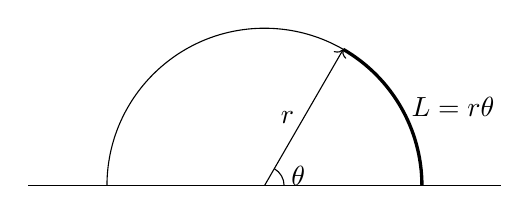
\begin{tikzpicture}
	% -- Semi-circle
	\draw[thin] (-3,0) -- (3,0);
	\draw[thin] (2,0) arc (0:180:2);

	% -- Arc
	\draw[thin,->] (0,0) -- (1,1.73) node[midway,left]{$r$};
	\draw[very thick] (2,0) arc (0:60:2) node[midway,right]{$L=r\theta$};

	% -- Angle measure
	\draw[thin] (0.25, 0) arc (0:60:0.25) node[midway,right]{$\theta$};
\end{tikzpicture}
\end{center}
By definition of radians:
\begin{equation*}
	\theta = \frac{L}{r}
\end{equation*}
For a more general curve with length element $\diff \vec{l}$, the element must be
projected onto the arc length $\diff L = \hat{r} \cdot \diff \vec{l}$:
\begin{equation*}
	\diff \theta = \frac{\hat{r} \cdot \diff \vec{l}}{r}
\end{equation*}

The solid angle is defined analagously, except with respect to the surface of a sphere:
\begin{equation*}
	\diff \Omega = \frac{\hat{r} \cdot \diff \vec{A}}{r^2} = \sin\theta \diff \theta \diff \phi
\end{equation*}

% -------------------- Fourier Transformations

\section{Fourier Transformations}
Asymmetric definition:
\begin{equation*}
	f(x) = \frac{1}{2\pi} \int_{-\infty}^\infty \tilde{f}(k) e^{ikx} \diff k \qquad \qquad \mathcal{F}[f](k) = \tilde{f}(k) = \int_{-\infty}^\infty f(x) e^{-ikx} \diff x
\end{equation*}

Symmetric definition:
\begin{equation*}
	f(x) = \frac{1}{\sqrt{2\pi}} \int_{-\infty}^\infty \tilde{f}(k) e^{ikx} \diff k \qquad \qquad \mathcal{F}[f](k) = \tilde{f}(k) = \frac{1}{\sqrt{2\pi}} \int_{-\infty}^\infty f(x) e^{-ikx} \diff x
\end{equation*}

\subsection{Convolution Theorem}
A \textbf{convolution} of two functions $f$ and $g$ is:
\begin{equation*}
	(f * g)(x) = \int_{-\infty}^\infty f(x') g(x-x') \diff x'
\end{equation*}

Fourier transformations turn convolutions in $x$-space to products in $k$-space:
\begin{equation*}
\begin{split}
	\mathcal{F}[f * g](k)
		&= \int_{-\infty}^\infty \diff x \int_{-\infty}^\infty \diff x' \, f(x')g(x-x') e^{-ikx} \\
		&= \int_{-\infty}^\infty \diff x' \, f(x')e^{-ikx'} \int_{-\infty}^\infty \diff x \, g(x-x') e^{-ik(x-x')} \\
		&= \mathcal{F}[f](k) \cdot \mathcal{F}[g](k) \\
\end{split}
\end{equation*}


\end{document}
